\documentclass[Royal,times,sageh]{sagej}

\usepackage{moreverb,url,natbib, multirow, tabularx}
\usepackage[colorlinks,bookmarksopen,bookmarksnumbered,citecolor=red,urlcolor=red]{hyperref}



% tightlist command for lists without linebreak
\providecommand{\tightlist}{%
  \setlength{\itemsep}{0pt}\setlength{\parskip}{0pt}}



\usepackage[linesnumbered,lined,boxed,commentsnumbered]{algorithm2e}
\usepackage{booktabs}
\usepackage{longtable}
\usepackage{array}
\usepackage{multirow}
\usepackage{wrapfig}
\usepackage{float}
\usepackage{colortbl}
\usepackage{pdflscape}
\usepackage{tabu}
\usepackage{threeparttable}
\usepackage{threeparttablex}
\usepackage[normalem]{ulem}
\usepackage{makecell}
\usepackage{xcolor}


\begin{document}


\setcitestyle{aysep={,}}

\title{A geo-referenced micro-data set of real estate listings for
Spain's three largest cities}

\runninghead{Rey-Blanco \emph{et al}.}

\author{D. Rey-Blanco\affilnum{1}, P. Arbues\affilnum{1}, F.
López\affilnum{2}, A. Páez*\affilnum{3}}

\affiliation{\affilnum{1}{Idealista, Plaza de las Cortes 5, 28014
Madrid, Spain}\\\affilnum{2}{Facultad de CC de la Empresa, C/ Real, 3.
30201 Cartagena, Murcia, Spain}\\\affilnum{3}{School of Earth,
Environment and Society, McMaster University, 1280 Main St W, Hamilton,
Ontario L8S 4K1 Canada}}

\corrauth{Antonio Páez, School of Earth, Environment and Society,
McMaster University, 1280 Main St W, Hamilton, Ontario L8S 4K1 Canada.}

\email{\href{mailto:paezha@mcmaster.ca}{\nolinkurl{paezha@mcmaster.ca}}}

\begin{abstract}
This article shares an open data product with big geo-referenced
micro-data sets of 2018 real estate listings in Spain. These data were
originally published on the idealista.com real estate website. The
observations were obtained for the three largest cities in Spain: Madrid
(n = 94,815 observations), Barcelona (n = 61,486 observations), and
Valencia (n = 33,622 observations). The data sets include the
coordinates of properties (latitude and longitude), asking prices of
each listed dwelling, and several variables of indoor characteristics.
The listings were enriched with official information from the Spanish
cadastre (e.g., building material quality) plus other relevant
geographical features, such as distance to urban points of interest.
Along with the real estate listings, the data product also includes
neighborhood boundaries for each city. The data product is offered as a
fully documented R package and is available for scientific and
educational purposes, particularly for geo-spatial studies
\end{abstract}

\keywords{Housing market; idealista.com; geo-referenced data;
point-level data; open data; Spain}

\maketitle

\hypertarget{introduction}{%
\section{Introduction}\label{introduction}}

Interest in the characteristics of the housing market and housing prices
has been a growing area of research in recent decades, generating a vast
amount of theoretical and empirical literature. Including the spatial
component to analyze the real estate market and incorporating geographic
variables has significantly improved the understanding of this market.
But to really understand the characteristics of the housing market, it
is essential to have information/data at the point level. Therefore, it
is becoming common for spatial analysis of urban environments to be
developed with geo- referenced micro-data sets \citep{lopez2015}.
However, the availability of this type of open data at the point level
is limited, and not many data sets contain latitude/longitude
coordinates for each dwelling. In some cases, researchers have had to
resort to web scraping processes to obtain the large volumes of
information that permit robust analyses
\citep{gupta2022take, arbia2020spatial, Li2019, lopez2015}. These web
scraping processes can include missing data, download errors, duplicate
records, etc. Furthermore, the authors of this research do not generally
share the data sets.

We are also witnessing a growing interest in open data in geography and
data science \citep{arribasl2021editorial, arribas2021} using
reproducible or replicable research \citep{paez2021open}. But to work
openly in science, it is necessary to have free software and open data.
While great efforts have been made to make free software available to
researchers (e.g., R or Python), not much data is currently out in the
open. In the particular case of the real estate market, to our
knowledge, there are few open micro-data sets of housing markets
available \citep{Song2021}.

To overcome these limitations, this paper presents a sort description of
an open micro-data set of geo-referenced dwelling listings. The data
have been provided by the Idealista
company\footnote{Idealista is the major real estate listing website in Spain, and present in other southern european countries as Italy and Portugal}
and contain information about 189,923 dwellings located in Spain's three
largest cities. To date, this data product is the biggest open
geo-referenced micro-data set of the housing market in Spain. Moreover,
the data set has been supplied directly by Idealista, and therefore is
clean and free of download errors. The listings have been enriched with
official information from the Spanish cadastre along with other relevant
geographical features, such as distance to urban points of interest. The
data set is distributed as an R package, named `idealista18', which can
be accessed from the Github
repository\footnote{The direct URL to the GitHub repository is \url{https://github.com/paezha/idealista18}}.

\hypertarget{data-description}{%
\section{Data description}\label{data-description}}

The open data set `idealista18' is an R package composed of nine
objects, three objects for each of the three main Spanish cities:
Barcelona, Madrid, and Valencia. For each city, dwelling listings,
neighborhood polygons, and a set of points of interest have been
included in the R package. The following subsections describe each
object. A full description of the data is available in the help section
of the package.

\hypertarget{dwelling-listings}{%
\subsection{Dwelling listings}\label{dwelling-listings}}

The dwelling listing of each city includes a set of characteristics for
each dwelling published on the idealista real estate website as an ad.
The dwelling listing has been included in the `idealista18' package as
an sf object \citep{Pebesma}. The name of the sf object containing the
dwelling listing includes the name of the city, followed by '\_Sale'
(e.g., Madrid\_Sale) and includes a total of 42 variables. Each sf
object includes the complete set of listings corresponding to the four
quarters of the year 2018. Table \ref{tab:number-ads} shows the number
of dwelling listing ads included in the data set for each city and
quarter. The record counts for each city are: 94,815 listings for
Madrid, 61,486 for Barcelona, and 33,622 for Valencia. Note that the
same dwelling may be found in more than one period when a property
listed for sale in one quarter was sold in a subsequent quarter. The
variable ASSETID, included in the sf objects, is the unique identifier
of the dwelling.

\begin{table}[ht]
\centering
\begin{tabular}{>{\raggedright\arraybackslash}p{4em}>{\raggedleft\arraybackslash}p{3em}cccc}
  \hline
City$\backslash$Quarter & First & Second  & Thirdr & Fourth & Total ads \\ 
  \hline
Barcelona & 17826 & 7951 & 12375 & 23334 & 61486 \\ 
  Madrid & 21920 & 12652 & 15973 & 44270 & 94815 \\ 
  Valencia & 9305 & 4655 & 5644 & 14018 & 33622 \\ 
   \hline
\end{tabular}
\caption{Number of dwelling  listing ads for each city and quarter. \label{tab:number-ads}} 
\end{table}

Each record of the dwelling listing contains a set of indoor
characteristics supplied by the advertisers on the Idealista website
(e.g., price, surface area, number of bedrooms, basic features, etc.),
including the exact location of the dwelling (see Section
\protect\hyperlink{anonymizing}{Anonymizing the data set}). Table
\ref{tab:variables} lists the main indoor variables with a short
description and the mean value of each variable. The dwelling listings
were enriched with a number of additional attributes from the Spanish
cadastre \citep{Catastro}. The cadastral information is described in
Table \ref{tab:variables}, with the prefix CAD in the variable name. The
cadastral features were assigned by applying the features of the nearest
parcel to the coordinates. The year the dwelling was built
(CONSTRUCTIONYEAR) given by the advertiser was revised since the year of
construction is entered on the website by users, and it is therefore
subject to errors and incomplete data (40\% missing data). To resolve
this issue, an alternative variable (CADCONSTRUCTIONYEAR) was included,
assigning the cadastral construction year from the nearest cadastral
parcel whenever the value was outstanding (date was after publication
date or year of construction was before 1500) or when the value supplied
by the advertiser was missing.

Additionally, the distance of each dwelling to three urban points of
interest was included in the sf object: distance to the city center,
distance to the closest metro station, and distance to a major street
(La Diagonal for Barcelona, La Castellana for Madrid, and Blasco Ibañez
for Valencia). The last rows of Table \ref{tab:variables} show the mean
values of these variables.

\begin{table}[ht]
\centering
\fontsize{8}{10}\selectfont
\begin{tabular}{>{\raggedright\arraybackslash}p{13em}>{\raggedright\arraybackslash}p{14em}ccc}
  \hline
Variable & Sort Description & Barcelona & Madrid & Valencia \\ 
  \hline
PRICE & Asking price & 395770.58 & 396110.11 & 199678.31 \\ 
  UNITPRICE & Asking price per m\verb|^|2 (euros) & 4044.86 & 3661.05 & 1714.54 \\ 
  CONSTRUCTEDAREA & Surface (m\verb|^|2) & 95.46 & 101.40 & 108.95 \\ 
  ROOMNUMBER & Number of bedrooms & 2.86 & 2.58 & 3.07 \\ 
  BATHNUMBER & Number of bathrooms & 1.52 & 1.59 & 1.59 \\ 
  CONSTRUCTIONYEAR & Construction year (advertiser) & 1952.58 & 1964.69 & 1969.43 \\ 
  CADCONSTRUCTIONYEAR & Construction year (cadastre) & 1952.19 & 1965.70 & 1970.55 \\ 
  CADMAXBUILDINGFLOOR & Max build floor & 6.85 & 6.38 & 7.04 \\ 
  CADDWELLINGCOUNT & Dwelling count in the building & 28.56 & 39.19 & 36.83 \\ 
  CADASTRALQUALITYID & Cadastral quality. 0 Best-10 Worst & 4.31 & 4.85 & 5.34 \\ 
  DISTANCE\_TO\_CITY\_CENTER & Distance to city center & 2.80 & 4.49 & 2.09 \\ 
  DISTANCE\_TO\_METRO & Distance to subway station & 0.27 & 0.48 & 0.64 \\ 
  DISTANCE\_TO\_(MAINSTREET) & Distance to major street & 1.77 & 2.68 & 2.07 \\ 
   \hline
\end{tabular}
\caption{List, sort description, and mean of the main quantitative variables included in the dwelling listing for the three Spanish cities. See the help section in the \textbf{idealista18} R package for details and formal definitions. Some variables have been excluded from this table to save space. Check the full list in the \textbf{idealista18} package.\label{tab:variables}} 
\end{table}

In addition to the variables listed in Table \ref{tab:variables}, the sf
object includes a set of dummy variables with information about the
basic characteristics of the dwelling. Table \ref{tab:Dummy-variables}
shows the more relevant variables included in the sf object.

\begin{table}[ht]
\centering
\fontsize{8}{10}\selectfont
\begin{tabular}{>{\raggedright\arraybackslash}p{12em}>{\raggedright\arraybackslash}p{14em}ccc}
  \hline
Variable & Sort Description & Barcelona & Madrid & Valencia \\ 
  \hline
HASTERRACE & =1 if has terrace & 0.33 & 0.36 & 0.25 \\ 
  HASLIFT & =1 if has lift & 0.74 & 0.70 & 0.79 \\ 
  HASAIRCONDITIONING & =1 if has air conditioning & 0.47 & 0.45 & 0.47 \\ 
  HASPARKINGSPACE & =1 if has parking & 0.08 & 0.23 & 0.17 \\ 
  HASNORTHORIENTATION & =1 if has north orientation & 0.13 & 0.11 & 0.13 \\ 
  HASSOUTHORIENTATION & =1 if has south orientation & 0.31 & 0.24 & 0.19 \\ 
  HASEASTORIENTATION & =1 if has east orientation & 0.24 & 0.20 & 0.25 \\ 
  HASWESTORIENTATION & =1 if has west orientation & 0.16 & 0.15 & 0.15 \\ 
  HASBOXROOM & =1 if has boxroom & 0.12 & 0.26 & 0.13 \\ 
  HASWARDROBE & =1 if has wardrobe & 0.30 & 0.57 & 0.53 \\ 
  HASSWIMMINGPOOL & =1 if has swimmingpool & 0.03 & 0.15 & 0.07 \\ 
  HASDOORMAN & =1 if has doorman & 0.08 & 0.25 & 0.05 \\ 
  HASGARDEN & =1 if has garden & 0.04 & 0.18 & 0.06 \\ 
  ISDUPLEX & =1 if is duplex & 0.03 & 0.03 & 0.02 \\ 
  ISSTUDIO & =1 if is studio & 0.02 & 0.03 & 0.01 \\ 
  ISINTOPFLOOR & =1 is on the top floor & 0.02 & 0.02 & 0.01 \\ 
  BUILTTYPEID\_1 & =1 if is new contruction & 0.01 & 0.03 & 0.03 \\ 
  BUILTTYPEID\_2 & =1 is second hand to be restored & 0.17 & 0.19 & 0.13 \\ 
  BUILTTYPEID\_3 & =1 is second hand in good condition & 0.82 & 0.78 & 0.83 \\ 
   \hline
\end{tabular}
\caption{List of dummy variables, sort description, and ratios of dwellings with the specific characteristics. See the help section in the \textbf{idealista18} R package for details and formal definitions. Some dummy variables have been excluded from this table to save space\label{tab:Dummy-variables}} 
\end{table}

\hypertarget{neighboorhood-polygons}{%
\subsection{Neighboorhood polygons}\label{neighboorhood-polygons}}

The second block of data included in the `idealista18' R package is the
spatial features of the three cities divided into neighborhoods. There
is an sf object for each city with the name of the city and the suffix
'\_Polygons'. Figure \ref{fig:all-polygons} shows the quantile maps of
the number of dwellings in the listing for the different neighborhoods
in the three cities. The neighborhoods are based on the official
boundaries but slightly changed by
Idealista\footnote{There are two criteria used to make this division. If an area is small enough and similar enough to another, the two areas are merged, and, if the official area is not homogeneous, it is divided into a series of new polygons.}.
In practical terms, we can assume they are the same since the website
combines areas when there are few ads for that area. In the case of
Madrid, they combined four areas into two.

\begin{figure}
\centering
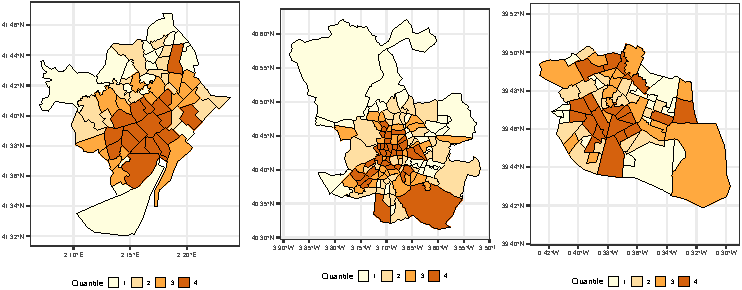
\includegraphics{EPB_files/figure-latex/unnamed-chunk-1-1.pdf}
\caption{\label{fig:all-polygons}Quantile maps of the number of
dwellings in each neighborhood. Boundary for Barcelona (Left), Madrid
(Center), and Valencia (Right).}
\end{figure}

There are a total of 69 neighborhoods in Barcelona, 135 in Madrid, and
73 in Valencia. The sf object includes a unique identifier (LOCATIONID)
and the neighborhood name (LOCATIONNAME).

\hypertarget{points-of-interest}{%
\subsection{Points of Interest}\label{points-of-interest}}

The last block of data included in the data package is a set of Points
of Interest in each city as an object of the class list. The name of the
list includes the name of the city with the suffix '\_POIS'. These lists
include three elements: (i) the coordinates of the city center, the
central business district; (ii) a set of coordinates that define the
main street of each city; and (iii) the coordinates of the metro
stations.

\hypertarget{anonymizing}{%
\section{Anonymizing the data set}\label{anonymizing}}

To comply with Spanish regulations, two variables were slightly modified
to provide anonymity. A masking process was applied to asking prices and
location (coordinates).

In terms of the asking prices, the original values were obfuscated with
the addition or subtraction of a random percentage of their original
values, ranging from -2.5\% to +2.5\%. Since asking prices are usually
multiples of 1,000, after the first price modification, the prices were
aligned to multiples of 1,000.

\begin{algorithm}[!ht]
 \KwData{all idealista listings}
 \KwResult{all idealista listings with masked coordinates}
 initialization\;
 \For{each listing L}{
  take geographical location of L as $(X,Y)$
  \Repeat{this stop condition}{
    take a random angle $\alpha$ from 0 to 360 degrees
    take a distance $R$ as a random value from 30 to 60 meters
    determine a new point $(X',Y')$ calculated as a point located $R$ with the angle $\alpha$
  }
  set $(X',Y')$ as the new location for the listing L
 }
 \caption{Coordinate displacement process for anonymisation purposes}
 \label{algo:coordinates-displacement}
\end{algorithm}

With respect to the location of the dwelling, a spatial masking process
was implemented to maintain the spatial properties of the original data
set. The coordinates of each listing were displaced using a stochastic
procedure. The listings were recorded using coordinates contained in
maximum and minimum displacement circles, as shown in Figure
\ref{fig:Anonymizing} (left). To preserve inclusion in a neighborhood,
the spatial masking procedure was constrained to ensure that the masked
coordinates remained in the original neighborhood of the listing.

Algorithm \ref{algo:coordinates-displacement} iteratively displaces the
coordinates of each listing with a minimum distance and a maximum
distance with the restriction that the new coordinates do not fall into
a different neighborhood. This ensures that neighborhood attributes are
preserved.

Figure \ref{fig:Anonymizing} (right) shows the histogram of the
displacements in meters for all the listings in the city of Valencia.
The average distance between the original and masked coordinates is 45
meters.

\begin{figure}

{\centering 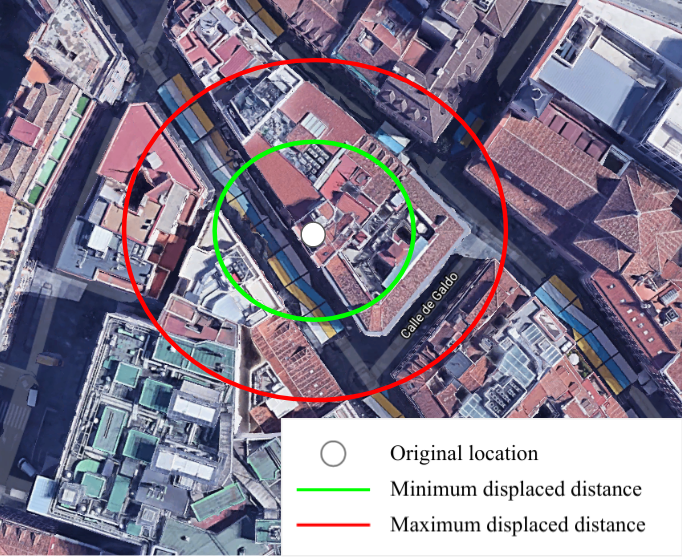
\includegraphics[width=0.29\linewidth,height=0.2\textheight]{EPB_files/points-moved-image} 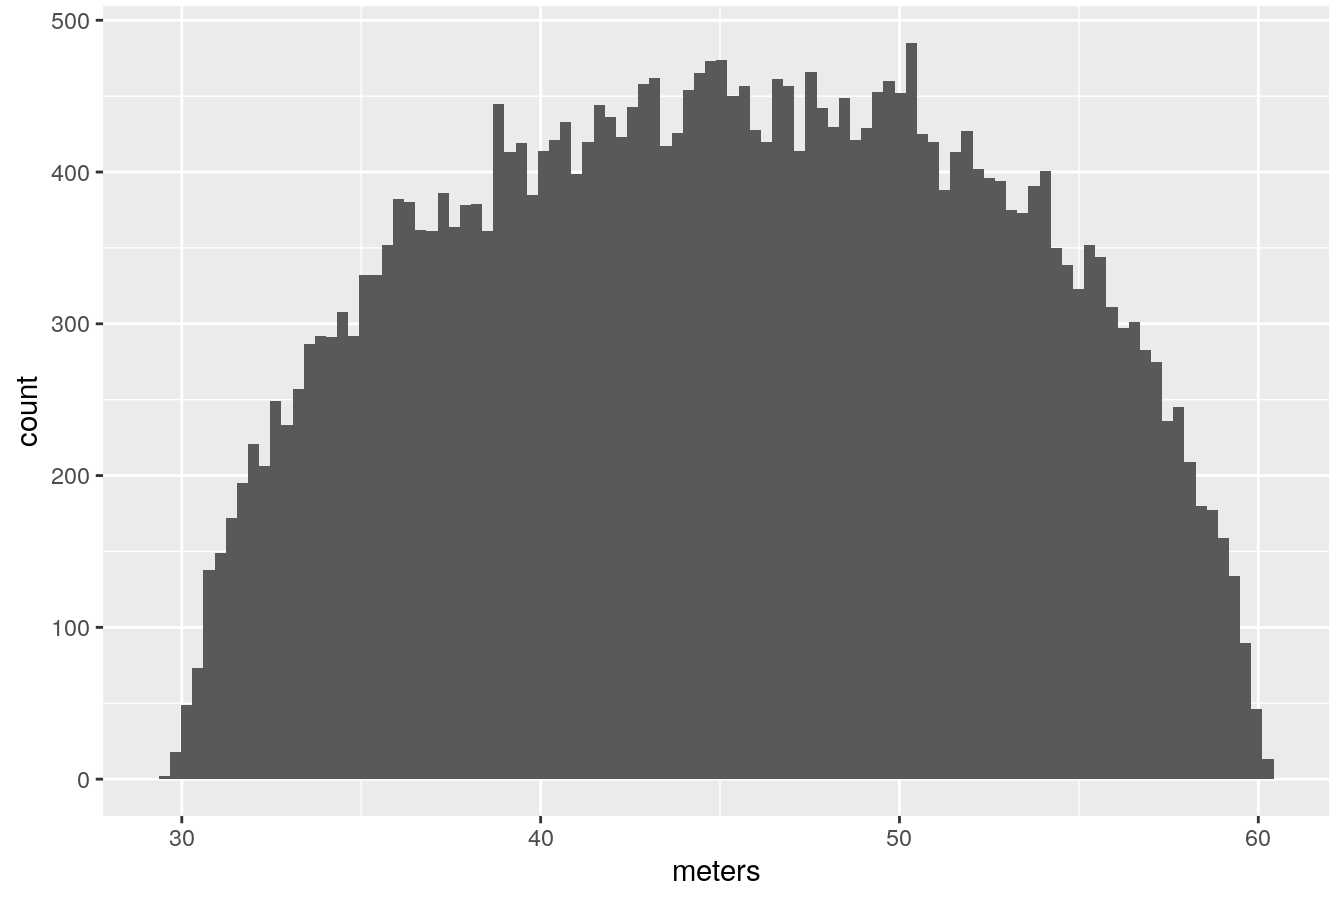
\includegraphics[width=0.37\linewidth,height=0.2\textheight]{EPB_files/coordinates-valencia} 

}

\caption{\label{fig:Anonymizing}(Left) Masking coordinates. Spatial range. (Right) Coordinate displacement in meters (Valencia)}\label{fig:unnamed-chunk-2}
\end{figure}

\hypertarget{conclusion}{%
\section{Conclusion}\label{conclusion}}

This paper describes a data product of a geo-referenced micro-data set
of Spain's three largest cities. This is an excellent data product to
help understand the complex mechanisms related to the housing market and
housing prices. Researchers can apply hedonic models with spatial
effects, identifying housing submarkets or machine learning techniques.
The data product can also be used for educational proposes and teaching
activities.

\hypertarget{declaration-of-competing-interest}{%
\section{Declaration of Competing
Interest}\label{declaration-of-competing-interest}}

Author One and author Two are employed by Idealista. They have been
granted permission to share the data presented in this article. None of
the authors have financial interests or personal relationships which
have, or could be perceived to have, influenced the work reported in
this article.

\hypertarget{acknowledgments}{%
\section{Acknowledgments}\label{acknowledgments}}

The authors wish to thank Alessandro Galesi for their support in the
paper revision and Juan Ramón Selva for collecting and cleaning the
spatial data. This work has been partially funded by the Spanish
Ministry of Economy and Competitiveness Grants PID2019-107800GB-100

\bibliographystyle{sageh}
\bibliography{bibEPB.bib}


\end{document}
